\chapter{Specifikacija programske potpore}
		
	\section{Funkcionalni zahtjevi}
			
			
			\noindent \textbf{\\Dionici:}
			
			\begin{packed_enum}
				\item Vlasnik sustava (direktor poduzeća/naručitelj)
				\item Djelatnici poduzeća
				\begin{itemize}
					\item Voditelji grupa
					\item Ostali djelatnici
				\end{itemize}
				\item Razvojni tim
			\end{packed_enum}
			
			\noindent \textbf{Aktori i njihovi funkcionalni zahtjevi:}
			\begin{packed_enum}
				\item  \underbar{Vlasnik sustava (direktor poduzeća) može:}
				
				\begin{packed_enum}
					\item definirati uslužne djelatnosti koje će poduzeće raditi
					\item dodijeliti djelatnosti voditeljima grupa
					\item registrirati novog djelatnika (uključujući i voditelja grupa) i pritom mu dodijeliti ulogu
					\item vidjeti zauzetost i realizaciju za sve djelatnike
					\item vidjeti trenutno i prošlu poticiju svih djelatnika koji su izašli na intervencije na karti
				\end{packed_enum}
			
				\item  \underbar{Voditelji grupa mogu:}
				
				\begin{packed_enum}
					\item definirati zadatke i dodjeljivati ih djelatnicima
					\item zabilježiti procjenu radnih sati potrebnih za zadatak
					\item odrediti cijenu sata rada ovisno o djelatnosti ili zadatku
					\item pregledati podatke za sebe i svoju grupu
					\item upisati broj odrađenih sati za svaki dan
				\end{packed_enum}
				\eject
				\item  \underbar{Ostali djelatnici mogu:}
				\begin{packed_enum}
					\item vidjeti koji su mu zadaci dodijeljeni i u kojim se grupama nalazi
					\item pregledati vlastite podatke
					\item upisati broj odrađenih radnih sati za svaki dan
				\end{packed_enum}
			
			\item  \underbar{Neregistrirani korisnik može:}
			\begin{packed_enum}
				\item vidjeti popis i opis djelatnosti poduzeća
			\end{packed_enum}
			\end{packed_enum}
			
			\eject 

			\subsection{Obrasci uporabe}
				
				
				\subsubsection{Opis obrazaca uporabe}
				%	
					\noindent \underbar{\textbf{UC1 - Pregled djelatnosti}}
					\begin{packed_item}
	
						\item \textbf{Glavni sudionik: }Korisnik
						\item  \textbf{Cilj:} Pregledati djelatnosti koje poduzeće obavlja
						\item  \textbf{Sudionici:} baza podataka
						\item  \textbf{Preduvjet:} -
						\item  \textbf{Opis osnovnog tijeka:}
						
						\item[] \begin{packed_enum}
	
							\item Korisnik u aplikaciji odabire opciju "Prikaz djelatnosti"
							\item Prikaže se popis svih djelatnosti poduzeća
						\end{packed_enum}
					\end{packed_item}
				%
					\noindent \underbar{\textbf{UC2 - Pregled opisa djelatnosti}}
				\begin{packed_item}
					
					\item \textbf{Glavni sudionik: }Korisnik
					\item  \textbf{Cilj:} Pregledati opis djelatnosti koje poduzeće obavlja
					\item  \textbf{Sudionici:} baza podataka
					\item  \textbf{Preduvjet:} -
					\item  \textbf{Opis osnovnog tijeka:}
					
					\item[] \begin{packed_enum}
						
						\item Korisnik odabire djelatnost za koju želi vidjeti informacije
						\item Prikaže se stranica s opisom odabrane djelatnosti
					\end{packed_enum}
				\end{packed_item}
				%
						\noindent \underbar{\textbf{UC3 - Registracija korisnika}}
					\begin{packed_item}
						
						\item \textbf{Glavni sudionik: } Direktor
						\item  \textbf{Cilj:} Stvoriti korisnički račun za pristup sustavu
						\item  \textbf{Sudionici:} baza podataka
						\item  \textbf{Preduvjet:} -
						\item  \textbf{Opis osnovnog tijeka:}
						
						\item[] \begin{packed_enum}
							\item Direktor odabire opciju za registraciju novih korisnika
							\item Direktor unosi sve potrebne korisničke podatke
							\item Direktor novom korisniku dodjeljuje ulogu
							\item Direktor prima obavijest o uspješnoj registraciji
						\end{packed_enum}
						
						\item  \textbf{Opis mogućih odstupanja:}
						\item[] \begin{packed_item}
							\item[2.a] Odabir već zauzetog korisničkog imena i/ili elektroničke pošte, unos podataka u nedozvoljenom formatu ili upis neispravnog imena elektroničke pošte
							\item[] \begin{packed_enum}
								\item Sustav obavještava direktora o neuspjelom upisu i vraća ga na stranicu za registraciju
								\item Direktor mijenja potrebne podatke te završava unos ili odustaje od registracije
								
							\end{packed_enum}
						\end{packed_item}
					\end{packed_item}
				%
					\noindent \underbar{\textbf{UC4 - Prijava u sustav}}
				\begin{packed_item}
					\item \textbf{Glavni sudionik: }Djelatnik
					\item  \textbf{Cilj:} Dobiti pristup korisničkom sučelju
					\item  \textbf{Sudionici:} baza podataka
					\item  \textbf{Preduvjet:} Registracija
					\item  \textbf{Opis osnovnog tijeka:}
					\item[] \begin{packed_enum}
						\item Djelatnik odabire opciju za prijavu u sustav
						\item Djelatnik upisuje korisničko ime i lozinku
						\item Sustav potvrđuje ispravnost unesenih podataka
						\item Djelatnik dobiva pristup korisničkim funkcijama
					\end{packed_enum}
				
					\item  \textbf{Opis mogućih odstupanja:}
					\item[] \begin{packed_item}
						\item[2.a] Unos neispravnog imena i/ili lozinke
						\item[] \begin{packed_enum}
							\item Sustav obavještava korisnika o neispravnom upisu podataka i neuspjeloj prijavi te ga vraća na stranicu za prijavu
						\end{packed_enum}
					\end{packed_item}
				\end{packed_item}
				%
				\noindent \underbar{\textbf{UC5 - Pregled svih grupa }}
			\begin{packed_item}
				\item \textbf{Glavni sudionik: } Vlasnik sustava (direktor poduzeća)
				\item  \textbf{Cilj:} Pregledati sve postojeće grupe u poduzeću
				\item  \textbf{Sudionici:} baza podataka
				\item  \textbf{Preduvjet:} vlasnik je prijavljen
				\item  \textbf{Opis osnovnog tijeka:}
				\item[] \begin{packed_enum}
					\item Vlasnik odabire opciju "Pregled grupa"
					\item Vlasniku se prikazuje popis grupa
				\end{packed_enum}
			\end{packed_item}
			%
			\noindent \underbar{\textbf{UC6 - Stvaranje grupe}}
			\begin{packed_item}
			
			\item \textbf{Glavni sudionik: } Vlasnik sustava (direktor poduzeća)
			\item  \textbf{Cilj:} Stvoriti grupu djelatnika 
			\item  \textbf{Sudionici:} Baza podataka
			\item  \textbf{Preduvjet:} Vlasnik je prijavljen
			\item  \textbf{Opis osnovnog tijeka:}
			\item[] \begin{packed_enum}
				\item Vlasnik odabire opciju “Pregled grupa” 
				\item Vlasniku se prikazuje popis grupa 
				\item Vlasnik odabire opciju “Stvori novu grupu” 
				\item Vlasniku se prikazuje popis svih djelatnika  
				\item Vlasnik odabire djelatnike koji će biti raspodijeljeni u grupu 
				\item Vlasnik odabire opciju “Odaberi voditelja” 
				\item Vlasniku odabire jednoga od članova grupe s popisa kojega postavlja za voditelja 
				\item Vlasnik odabire opciju “Potvrđujem odabir” 
				\item Sustav javlja vlasniku da je grupa uspješno stvorena 
					\end{packed_enum}
			\end{packed_item}
			%
			\noindent \underbar{\textbf{UC7 -Uređivanje grupe}}
			\begin{packed_item}
				
				\item \textbf{Glavni sudionik: } Vlasnik
				\item  \textbf{Cilj:} Urediti članove grupe
				\item  \textbf{Sudionici:} baza podataka
				\item  \textbf{Preduvjet:} Vlasnik je prijavljen
				\item  \textbf{Opis osnovnog tijeka:}
				\item[] \begin{packed_enum}
					\item Vlasnik odabire opciju “Pregled grupa”
					\item Vlasniku se prikazuje popis grupa
					\item Vlasnik odabire grupu čije članove želi urediti
					\item Vlasnik odabire opciju “Uredi”
					\item Vlasnik uređuje članove grupe
				\end{packed_enum}
			\end{packed_item}
			%
			\noindent \underbar{\textbf{UC8 - Brisanje grupe}}
			\begin{packed_item}
				\item \textbf{Glavni sudionik: } Vlasnik
				\item  \textbf{Cilj:} Obrisati grupu
				\item  \textbf{Sudionici:} Baza podataka
				\item  \textbf{Preduvjet:} Vlasnik je prijavljen
				\item  \textbf{Opis osnovnog tijeka:}
				\item[] \begin{packed_enum}
					\item Vlasnik odabire opciju “Pregled grupa”
					\item Vlasniku se prikazuje popis grupa
					\item Vlasnik odabire grupu koju želi obrisati
					\item Vlasnik odabire opciju “Brisanje grupe”
					\item Vlasniku se prikazuje poruka “Jeste li sigurni da želite obrisati grupu?”
					\item Vlasnik odabire opciju “Da”
				\end{packed_enum}
			\end{packed_item}
			%
			\eject
			
			\noindent \underbar{\textbf{UC9 - Promjena voditelja grupe}}
			\begin{packed_item}
				\item \textbf{Glavni sudionik: } Vlasnik
				\item  \textbf{Cilj:} Promijeniti voditelja grupe
				\item  \textbf{Sudionici:} baza podataka
				\item  \textbf{Preduvjet:} Vlasnik je prijavljen
				\item  \textbf{Opis osnovnog tijeka:}
				\item[] \begin{packed_enum}
					\item Vlasnik odabire opciju “Pregled grupa”
					\item Vlasniku se prikazuje popis grupa
					\item Vlasnik odabire grupu kojoj želi promijeniti voditelja	
					\item Vlasnik odabire opciju “Promjena voditelja”
					\item Vlasniku se prikazuje popis članova grupe
					\item Vlasnik odabire člana grupe koji će biti novi voditelj grupe
				\end{packed_enum}
			\end{packed_item}
			%
			\noindent \underbar{\textbf{UC10 - Definiranje uslužne djelatnosti}}
			\begin{packed_item}
				\item \textbf{Glavni sudionik: } Vlasnik
				\item  \textbf{Cilj:} Definirati uslužnu djelatnost
				\item  \textbf{Sudionici:} baza podataka
				\item  \textbf{Preduvjet:} Vlasnik je prijavljen
				\item  \textbf{Opis osnovnog tijeka:}
				\item[] \begin{packed_enum}
					\item Vlasnik odabire opciju “Pregled djelatnosti”
					\item Vlasniku se prikazuje popis djelatnosti
					\item Vlasnik odabire opciju “Stvori djelatnost”
					\item Vlasnik ispuni obrazac za stvaranje djelatnosti
					\item Vlasnik odabire opciju “Potvrdi unos”
				\end{packed_enum}
				\item  \textbf{Opis mogućih odstupanja:}
				\item[] \begin{packed_item}
					\item[4.a] Neispunjena sva polja obrasca
					\item[] \begin{packed_enum}
						\item Sustav šalje poruku “Molimo vas ispunite sva polja obrasca.”
						\item Vlasnik ispunjava obrazac do kraja i ponovno ga potvrđuje
					\end{packed_enum}
				\end{packed_item}
			\end{packed_item}
			%
			\noindent \underbar{\textbf{UC11 - Dodjela djelatnosti (direktor voditeljima)}}
			\begin{packed_item}
				\item \textbf{Glavni sudionik: } Vlasnik
				\item  \textbf{Cilj:} Dodijeliti djelatnost voditelju grupe
				\item  \textbf{Sudionici:} baza podataka
				\item  \textbf{Preduvjet:} Vlasnik je prijavljen
				\item  \textbf{Opis osnovnog tijeka:}
				\item[] \begin{packed_enum}
					\item Vlasnik odabire opciju “Pregled grupa”
					\item Vlasniku se prikazuje popis grupa
					\item Vlasnik odabire grupu kojoj želi dodijeliti djelatnost
					\item Vlasnik odabere opciju “Dodijeli djelatnost”
					\item Vlasniku se prikazuje popis djelatnosti
					\item Vlasnik odabire djelatnost koju želi dodijeliti grupi
				\end{packed_enum}
				\item  \textbf{Opis mogućih odstupanja:}
				\item[] \begin{packed_item}
					\item[4.a] Neispunjena sva polja obrasca
					\item[] \begin{packed_enum}
						\item Sustav šalje poruku “Molimo vas ispunite sva polja obrasca.”
						\item Vlasnik ispunjava obrazac do kraja i ponovno ga potvrđuje
					\end{packed_enum}
				\end{packed_item}
			\end{packed_item}
			%
			\noindent \underbar{\textbf{UC12 - Dodjela zadataka (voditelji djelatnicima)}}
			\begin{packed_item}
				\item \textbf{Glavni sudionik: } voditelj grupe
				\item  \textbf{Cilj:} Dodijeliti djelatnost Razrada plana rada i dodjela zadataka pojedinim djelatnicima
				\item  \textbf{Sudionici:} baza podataka
				\item  \textbf{Preduvjet:} Korisnik je registriran i dodijeljena mu je uloga "voditelj grupe"
				\item  \textbf{Opis osnovnog tijeka:}
				\item[] \begin{packed_enum}
					\item Voditelj grupe odabire djelatnika koji će obavljati zadatak.
					\item Voditelj grupe dodjeljuje zadatak odabranom djelatniku.
					\item Upisani podaci se spremaju pritiskom na opciju “Spremi” 
					\item Zadaci postaju vidljivi pojedinim djelatnicima. 
				\end{packed_enum}
				\item  \textbf{Opis mogućih odstupanja:}
				\item[] \begin{packed_item}
					\item[2.a] Zauzetost djelatnika
					\item[] \begin{packed_enum}
						\item U trenutku dodjele zadatka odabranom djelatniku, ukoliko je već u tom vremenskom periodu istom zadan neki zadatak, sustav šalje poruku upozorenja o preklapanju. 
						\item Voditelj grupe zatim zadaje drugi termin djelatniku. 
					\end{packed_enum}
				\end{packed_item}
			\end{packed_item}
			%
			\noindent \underbar{\textbf{UC13 - Upis odrađenih sati}}
			\begin{packed_item}
				\item \textbf{Glavni sudionik: } djelatnici, voditelji grupa
				\item  \textbf{Cilj:} Praćenje odrađenih radnih sati u danu za svakog djelatnika.
				\item  \textbf{Sudionici:} baza podataka
				\item  \textbf{Preduvjet:} Prijava korisnika u sustav.
				\item  \textbf{Opis osnovnog tijeka:}
				\item[] \begin{packed_enum}
					\item Svaki djelatnik i voditelj grupa nakon radnog dana upiše odrađeno vrijeme (sati i minute) za taj dan.
					\item Uneseni podaci pohranjuju se u bazu klikom na gumb “Spremi”. 
				\end{packed_enum}
			\end{packed_item}
			%
			\noindent \underbar{\textbf{UC14 - Pregled dodijeljenih zadataka}}
			\begin{packed_item}
				\item \textbf{Glavni sudionik: djelatnik} 
				\item  \textbf{Cilj:} Pojedini djelatnik može vidjeti koji su mu zadaci dodijeljeni.
				\item  \textbf{Sudionici:} baza podataka
				\item  \textbf{Preduvjet:} Korisnik mora biti prijavljen u sustav i imati ulogu “djelatnika”.
				\item  \textbf{Opis osnovnog tijeka:}
				\item[] \begin{packed_enum}
					\item Djelatnik pristupa stranici dodijeljenih zadataka. 
					\item S obzirom da je djelatnik prijavljen u sustav, poznati su nam njegovi identifikacijski podaci te na temelju njih prikazuje se raspored samo za tog djelatnika. 
				\end{packed_enum}
			\end{packed_item}
			%
			\noindent \underbar{\textbf{UC15 - Prikaz dodijeljenih grupa}}
			\begin{packed_item}
				\item \textbf{Glavni sudionik: } djelatnik
				\item  \textbf{Cilj:} Pojedini djelatnik može vidjeti u kojim se grupama nalazi
				\item  \textbf{Sudionici:} baza podataka
				\item  \textbf{Preduvjet:} Korisnik mora biti prijavljen u sustav i imati ulogu “djelatnika”.
				\item  \textbf{Opis osnovnog tijeka:}
				\item[] \begin{packed_enum}
					\item Djelatnik odabire stranicu dodijeljenih grupa.
					\item Na temelju njegovih identifikacijskih oznaka prikazuju mu se dodijeljene grupe.
				\end{packed_enum}
			\end{packed_item}
			%
			\noindent \underbar{\textbf{UC16 - Pregled zauzetosti djelatnika}}
			\begin{packed_item}
				\item \textbf{Glavni sudionik: } djelatnik, voditelj grupe, direktor
				\item  \textbf{Cilj:} Korisnik može vidjeti predviđenu zauzetost djelatnika ovisno o ulozi. Direktor ima pristup zauzetosti svih djelatnika, voditelji grupe imaju pristup podacima za sebe i svoju grupu, a djelatnik može vidjeti samo podatke za sebe.
				\item  \textbf{Sudionici:} baza podataka
				\item  \textbf{Preduvjet:} Korisnik mora biti prijavljen u sustav.
				\item  \textbf{Opis osnovnog tijeka:}
				\item[] \begin{packed_enum}
					\item Korisnik, ako je direktor ili voditelj grupe odabire djelatnika čiju zauzetost želi provjeriti. 
					\item Odabire se vrijeme za koje se želi provjeriti zauzetost. 
					\item Na temelju identifikacijskih podataka odabranog djelatnika ili prijavljenog korisnika, ako je njegova uloga “djelatnik” ili “voditelj grupe”, prikazuje se zauzetost u prethodno navedenom vremenu.
				\end{packed_enum}
			\end{packed_item}
			%
			\noindent \underbar{\textbf{UC17 - Pregled realizacije djelatnika}}
			\begin{packed_item}
				\item \textbf{Glavni sudionik: } djelatnik, voditelj grupe, direktor
				\item  \textbf{Cilj:} Korisnik može vidjeti stvarnu i materijalnu realizaciju djelatnika, ovisno o njegovoj ulozi. Direktor ima pristup realizaciji svih djelatnika, voditelji grupe imaju pristup podacima za sebe i svoju grupu, a djelatnik može vidjeti samo podatke za sebe. 
				\item  \textbf{Sudionici:} baza podataka
				\item  \textbf{Preduvjet:} Prijava korisnika u sustav.
				\item  \textbf{Opis osnovnog tijeka:}
				\item[] \begin{packed_enum}
					\item Korisnik, ako je direktor ili voditelj grupe odabire djelatnika čiju realizaciju želi provjeriti. 
					\item Odabire se zadatak za koji se želi provjeriti realizacija. 
					\item Na temelju identifikacijskih podataka odabranog djelatnika ili  prijavljenog korisnika, ako je njegova uloga “djelatnik” ili “voditelj grupe”, prikazuje se realizacija za određeni zadatak.
				\end{packed_enum}
			\end{packed_item}
			%
			\noindent \underbar{\textbf{UC18 - Pregled odnosa planiranih i realiziranih troškova}}
			\begin{packed_item}
				\item \textbf{Glavni sudionik: } Direktor
				\item  \textbf{Cilj:} Evidencija financijskih rashoda.
				\item  \textbf{Sudionici:} baza podataka
				\item  \textbf{Preduvjet:} Korisnik mora biti prijavljen u sustav i imati ulogu “direktor”.
				\item  \textbf{Opis osnovnog tijeka:}
				\item[] \begin{packed_enum}
					\item Direktor unosi planirane troškove u bazu. 
					\item Tijekom obavljanja poslova, redovito se upisuju realizirani troškovi. 
					\item Sustav na temelju unesenih podataka računa razliku. 
					\item Prikazuje se odnos planiranih I realiziranih troškova.
				\end{packed_enum}
			\end{packed_item}
			%
			\eject
			\noindent \underbar{\textbf{UC19 - Pregled odnosa planiranih I realiziranih dobiti}}
			\begin{packed_item}
				\item \textbf{Glavni sudionik: } direktor
				\item  \textbf{Cilj:} Evidencija financijskih prihoda. 
				\item  \textbf{Sudionici:} baza podataka
				\item  \textbf{Preduvjet:} Korisnik prijavljen u sustav i ima ulogu “direktor”
				\item  \textbf{Opis osnovnog tijeka:}
				\item[] \begin{packed_enum}
					\item Direktor unosi planiranu dobit u bazu. 
					\item Tijekom obavljanja poslova, redovito se upisuju realizirane dobiti. 
					\item Sustav na temelju unesenih podataka računa razliku. 
					\item Prikazuje se odnos planiranih I realiziranih dobiti. 
				\end{packed_enum}
			\end{packed_item}
			%
			\noindent \underbar{\textbf{UC20 - Pregled podređene grupe (voditelj) }}
			\begin{packed_item}
				\item \textbf{Glavni sudionik: } Voditelj grupe
				\item  \textbf{Cilj:} Voditelj treba moći vidjeti članove grupe kojoj je on nadređen. Može vidjeti članove grupe, njihove podatke i dodijeljene zadatke.
				\item  \textbf{Sudionici:} baza podataka
				\item  \textbf{Preduvjet:} korisnik je prijavljen u sustav i ima ulogu “voditelj”
				\item  \textbf{Opis osnovnog tijeka:}
				\item[] \begin{packed_enum}
					\item Voditelj odabire opciju “Moje podređene grupe”. 
					\item Prikazuje se popis svih grupa kojima je taj voditelj nadređen. 
					\item Voditelj odabire grupu za koju želi vidjeti podatke. 
					\item Prikazuju se članovi grupe i djelatnost koja joj je dodijeljena. Odabirom pojedinog djelatnika prikazuju se njegovi podaci i dodijeljeni zadaci. 
				\end{packed_enum}
			\end{packed_item}
			%
			\noindent \underbar{\textbf{UC21 - Pregled vlastitih podataka}}
			\begin{packed_item}
				\item \textbf{Glavni sudionik: } direktor, voditelj grupe, djelatnik
				\item  \textbf{Cilj:} Svi djelatnici (uključujući i direktora i voditelje grupa) mogu vidjeti svoje osobne podatke, dodijeljene zadatke i grupe u kojima se nalazi. 
				\item  \textbf{Sudionici:} baza podataka
				\item  \textbf{Preduvjet:} Korisnik je prijavljen u sustav
				\item  \textbf{Opis osnovnog tijeka:}
				\item[] \begin{packed_enum}
					\item Korisnik odabire opciju “Moji podaci”. 
					\item Prikazuju se korisnikovi osobni podaci, njegovi dodijeljeni zadaci te grupe u kojima se nalazi.
				\end{packed_enum}
			\end{packed_item}
			%
			\eject
			\noindent \underbar{\textbf{UC22 - Unos lokacije aktivnosti izvan poduzeća}}
			\begin{packed_item}
				\item \textbf{Glavni sudionik: } voditelj grupe
				\item  \textbf{Cilj:} Voditelj treba stvoriti zadatak koji se obavlja izvan poduzeća 
				\item  \textbf{Sudionici:} baza podataka
				\item  \textbf{Preduvjet:} Voditelj je prijavljen u sustav
				\item  \textbf{Opis osnovnog tijeka:}
				\item[] \begin{packed_enum}
					\item Voditelj grupe odabire djelatnika koji će obavljati zadatak. 
					\item Voditelj grupe dodjeljuje zadatak izvan poduzeca odabranom djelatniku.
					\item Upisani podaci se spremaju pritiskom na opciju “Spremi” 
					\item Zadaci postaju vidljivi pojedinim djelatnicima. 
				\end{packed_enum}
				\item  \textbf{Opis mogućih odstupanja:}
				\item[] \begin{packed_item}
					\item[2.a] Zauzetost djelatnika
					\item[] \begin{packed_enum}
						\item U trenutku dodjele zadatka odabranom djelatniku, ukoliko je već u tom vremenskom periodu istom zadan neki zadatak, sustav šalje poruku upozorenja o preklapanju. 
						\item Voditelj grupe zatim zadaje drugi termin djelatniku. 
					\end{packed_enum}
				\end{packed_item}
			\end{packed_item}
			%
			\noindent \underbar{\textbf{UC23 - Pregled lokacija aktivnosti izvan poduzeća}}
			\begin{packed_item}
				\item \textbf{Glavni sudionik: } direktor
				\item  \textbf{Cilj:} Moguće je da djelatnici imaju aktivnosti koje moraju obaviti na nekoj lokaciji izvan poduzeća. U tom slučaju direktor mora moći vidjeti gdje su se nalazili. 
				\item  \textbf{Sudionici:} baza podataka
				\item  \textbf{Preduvjet:} korisnik je prijavljen u sustav i ima ulogu “direktor”
				\item  \textbf{Opis osnovnog tijeka:}
				\item[] \begin{packed_enum}
					\item Direktor odabire opciju “Pregledajte aktivnosti izvan poduzeća”. 
					\item Prikazuje se karta s označenim lokacijama aktivnosti. 
					\item Odabirom pojedine lokacije prikazuju se podaci o aktivnosti koja se obavljala na toj lokaciji I djelatniku koji je tu aktivnost obavljao. 
				\end{packed_enum}
			\end{packed_item}
			%
			\noindent \underbar{\textbf{UC24 - Pregled svih zaposlenika}}
			\begin{packed_item}
				\item \textbf{Glavni sudionik: } direktor
				\item  \textbf{Cilj:} Direktor mora moći vidjeti popis svih djelatnika poduzeća.
				\item  \textbf{Sudionici:} baza podataka
				\item  \textbf{Preduvjet:} korisnik je prijavljen i ima ulogu “direktor”
				\item  \textbf{Opis osnovnog tijeka:}
				\item[] \begin{packed_enum}
					\item Direktor odabire opciju “Popis djelatnika”. 
					\item Prikazuje se popis svih djelatnika I njihovih uloga. 
				\end{packed_enum}
			\end{packed_item}
			%
			\noindent \underbar{\textbf{UC25 - Uklanjanje zaposlenika}}
			\begin{packed_item}
				\item \textbf{Glavni sudionik: } direktor
				\item  \textbf{Cilj:} Broj djelatnika može se mijenjati, odnosno direktor mora imati mogućnost zapošljavanja i otpuštanja djelatnika. 
				\item  \textbf{Sudionici:} baza podataka
				\item  \textbf{Preduvjet:} korisnik je prijavljen i ima ulogu “direktor”
				\item  \textbf{Opis osnovnog tijeka:}
				\item[] \begin{packed_enum}
					\item Direktor odabire opciju “Popis djelatnika”. 
					\item Prikazuje se popis svih djelatnika i njihovih uloga. 
					\item Odabirom pojedinog djelatnika, osim njegovih podataka, prikazuje se I opcija “Otpusti djelatnika”. 
					\item Direktor potvrđuje da želi otpustiti djelatnika. 
					\item Djelatniku se uklanja status aktivnog zaposlenja. 
				\end{packed_enum}
			\end{packed_item}
			\eject
				\subsubsection{Dijagrami obrazaca uporabe\\}
					
				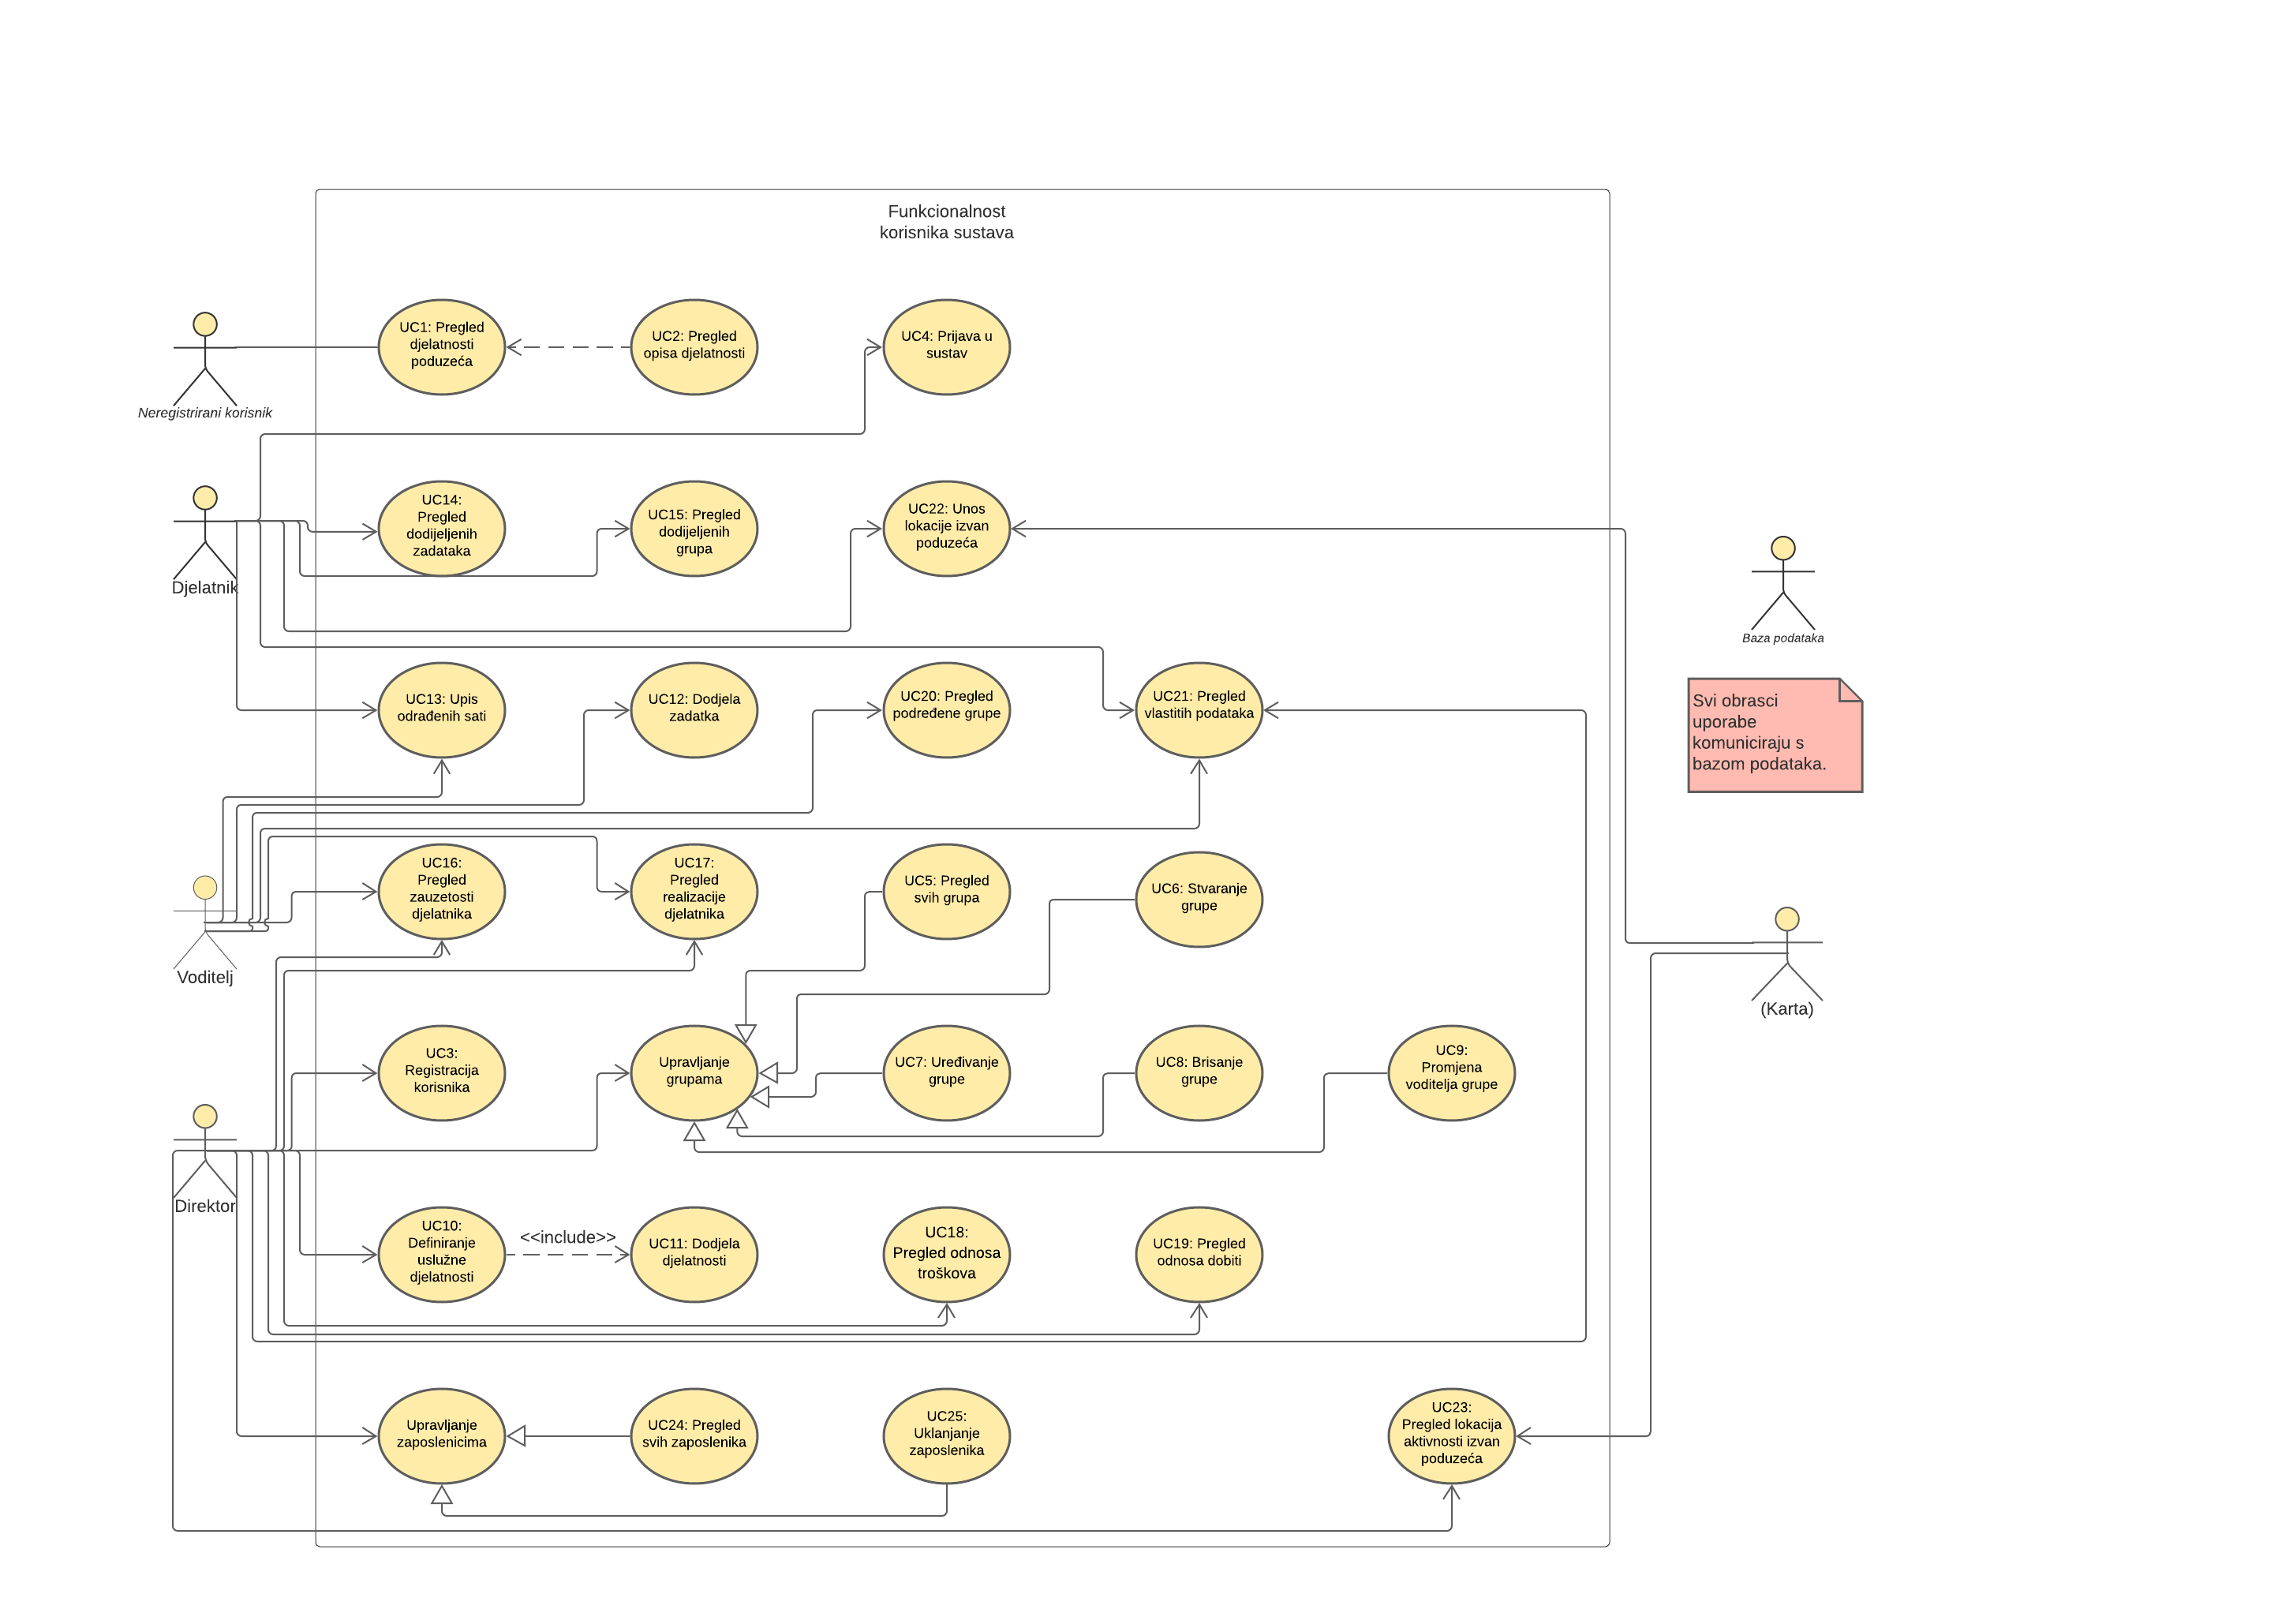
\includegraphics[width=1.25\textwidth]{Funkcionalnosti korisnika sustava}
				Slika 3.1 Funkcionalnosti korisnika sustava
				\eject		
				
			\subsection{Sekvencijski dijagrami}
				
				\noindent \textbf{UC3 – Registracija korisnika\\}
				Direktor otvara stranicu za registraciju djelatnika. Obavljanje zahtjeva obavlja se na poslužitelju koji kao odgovor vraća zatraženu stranicu. Direktor unosi sve potrebne korisničke podatke za stvaranje potpuno novog profila djelatnika. Prilikom registracije direktor također dodjeljuje ulogu djelatniku. Tijekom unosa moguće su sljedeća odstupanja: već zauzeto korisničko ime i/ili elektronička pošta, unos podataka u neispravnom formatu (ilegalni znakovi, predugačak unos ili unos krivog tipa podataka). Ukoliko dođe do pogreške prilikom unosa, poslužitelj obavještava direktora o neuspjelom zahtjevu i vraća ga na stranicu za registraciju. U takvom slučaju direktor ispravlja unos te ponovno pokušava izvršiti unos ili odustaje od registracije. Svi uneseni podaci šalju se na poslužitelj te se spremaju u bazu podataka. Direktor prima obavijest o uspješnoj registraciji.\\
				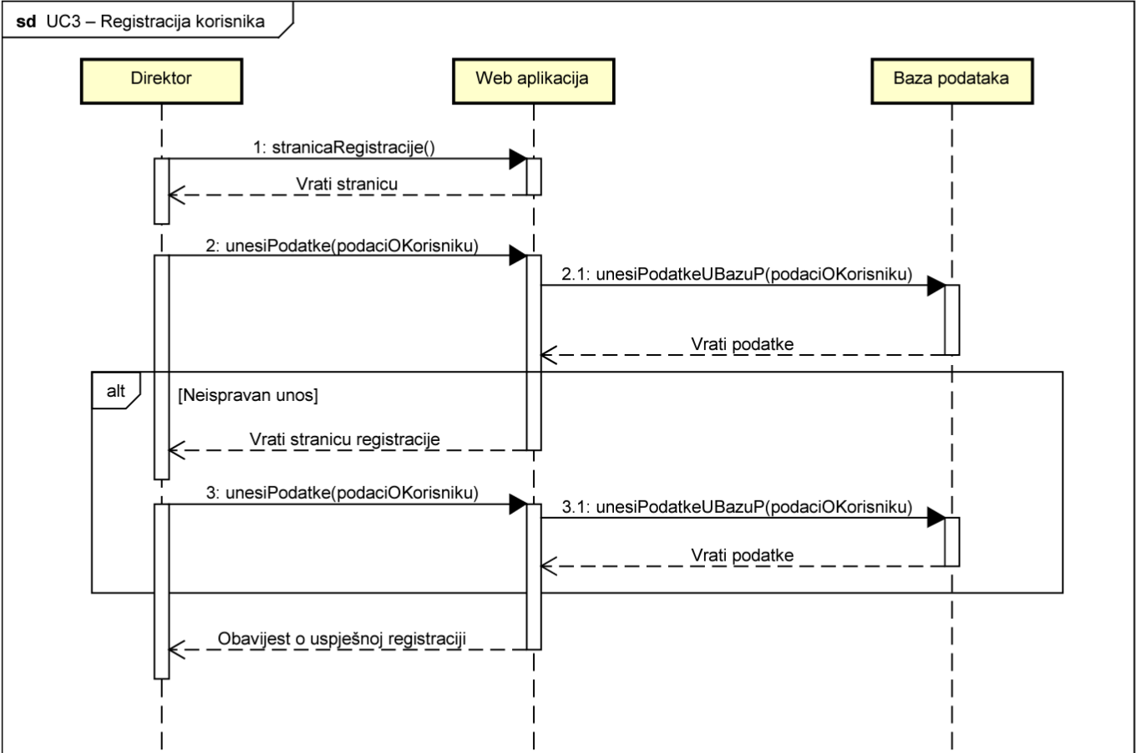
\includegraphics[width=\textwidth]{UC3}\\
				Slika 3.2 Registracija korisnika
				\eject
				\noindent \textbf{UC7 - Uređivanje grupe\\}
				Direktor odabire opciju “Pregled grupa”. Poslužitelj šalje zahtjev bazi, koja vraća popis grupa. Poslužitelj vraća prikaz sa popisom grupa direktoru. Zatim direktor odabire određenu grupu. Poslužitelj taj zahtjev šalje za određenu tablicu u bazi. Baza vraća određenu grupu stranici, a poslužitelj vraća popis ljudi u grupi iz baze direktoru. Direktor odabire opciju uredi. Poslužitelj prelazi u način uređivanja te se takva prikazuje direktoru. Direktor mijenja članove grupe*. Poslužitelj prosljeđuje zahtjev bazi. Baza mijenja članove grupe* . Baza vraća ažuriranu grupu web stranici. Poslužitelj prikazuje novi popis članova direktoru. 
				
				* Mijenjanje članova podrazumijeva brisanje, dodavanje te zamjenu (dupla operacija).\\
				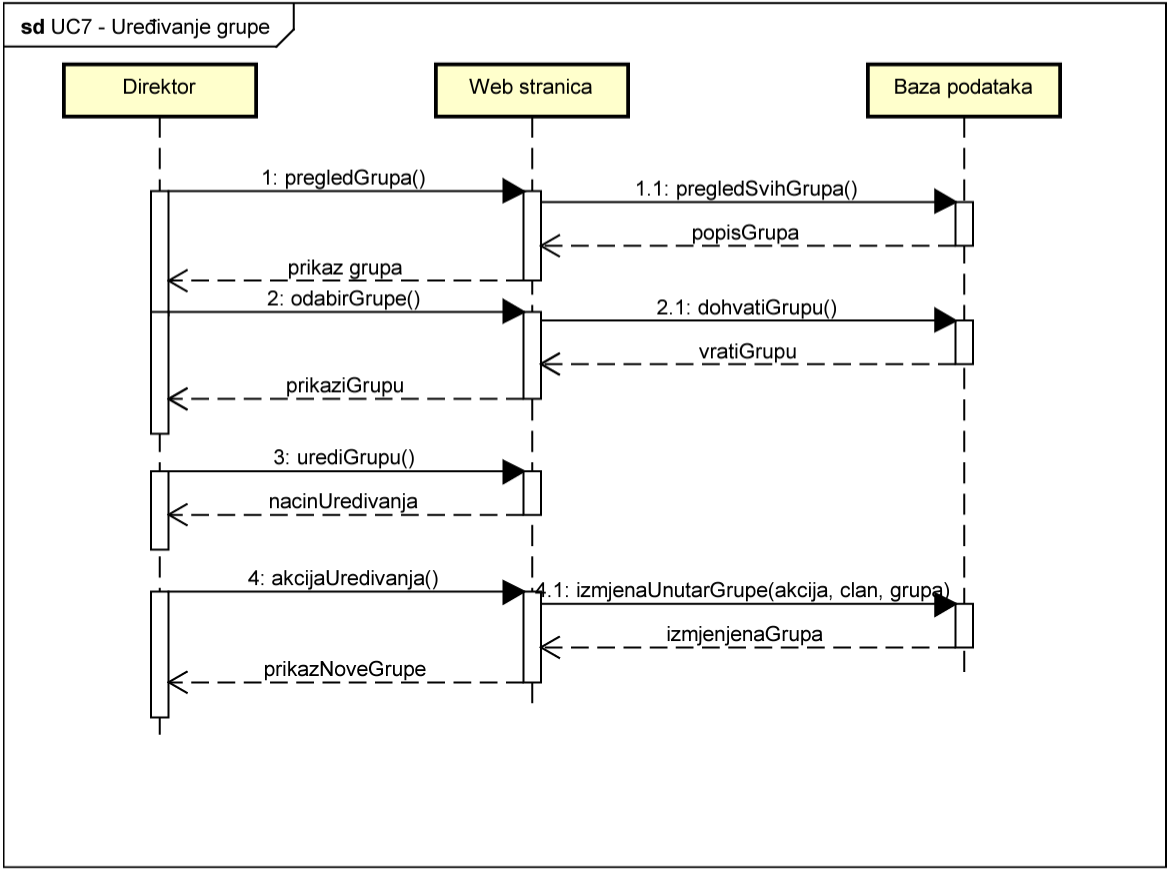
\includegraphics[width=\textwidth]{UC7}\\
				Slika 3.3 Uređivanje grupe
				\eject
				\noindent \textbf{UC11 – Dodjela djelatnosti (direktor voditeljima)\\}
				Direktor odabire opciju “Pregled grupa”. Poslužitelj šalje zahtjev bazi, koja vraća popis grupa. Poslužitelj vraća prikaz sa popisom grupa direktoru. Zatim direktor odabire određenu grupu. Poslužitelj taj zahtjev šalje za određenu tablicu u bazi. Baza vraća određenu grupu stranici, a poslužitelj vraća popis ljudi u grupi iz baze direktoru. Na prikazu grupe, direktor odabire opciju “Dodijeli djelatnost” *. Poslužitelj bazi šalje zahtjev za dohvaćanje popisa djelatnosti. Baza vraća poslužitelju taj popis. Poslužitelj prikazuje direktoru mogući odabir djelatnosti. Direktor odabire neku djelatnost. Poslužitelj prosljeđuje taj zahtjev bazi za odabranu grupu te postavlja djelatnost te grupe. Baza vraća ažuriranu djelatnost odabrane grupe. Poslužitelj vraća prikaz ažurirane djelatnosti na odabranoj grupi direktoru.  
				*Po završetku odabira djelatnosti, direktor može nastaviti mijenjati djelatnost od ovog koraka.\\ 
				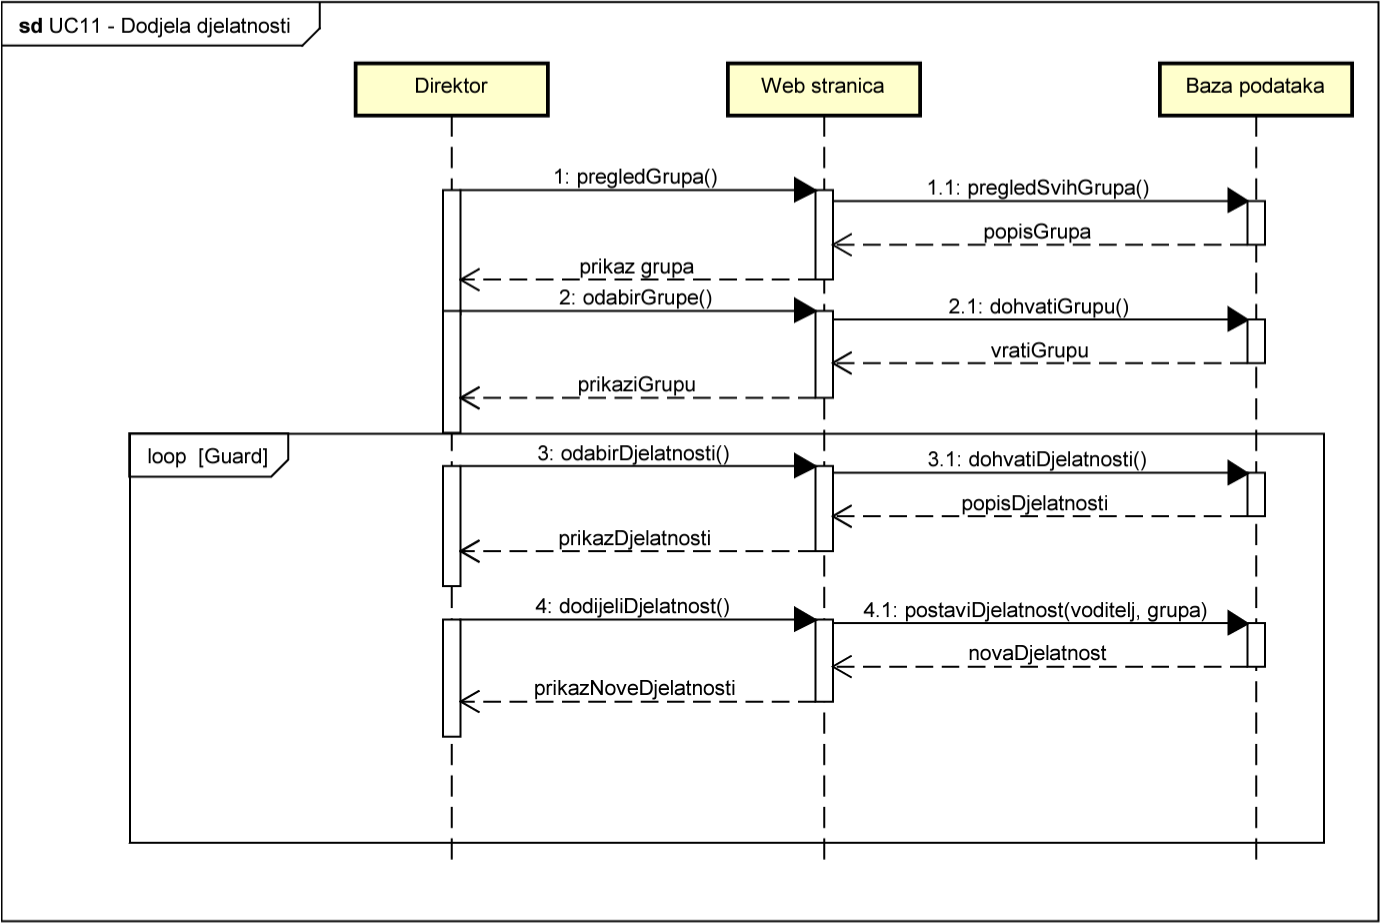
\includegraphics[width=\textwidth]{UC11}\\
				Slika 3.4 Dodjela djelatnosti
				\eject
				\noindent \textbf{UC22 – Unos lokacije aktivnosti izvan poduzeća\\}
				Djelatnik šalje poslužitelju zahtjev za unos aktivnosti izvan poduzeća. Na web pregledniku otvara se obrazac za upis adrese na kojoj je djelatnik obavljao aktivnost. Podaci se šalju pregledniku te se dohvaća karta s prikazom navedene adrese. Karta se prikazuje djelatniku. Djelatnik potvrđuje lokaciju pritiskom na gumb “Potvrdi” te se adresa upisuje u bazu podataka.\\
				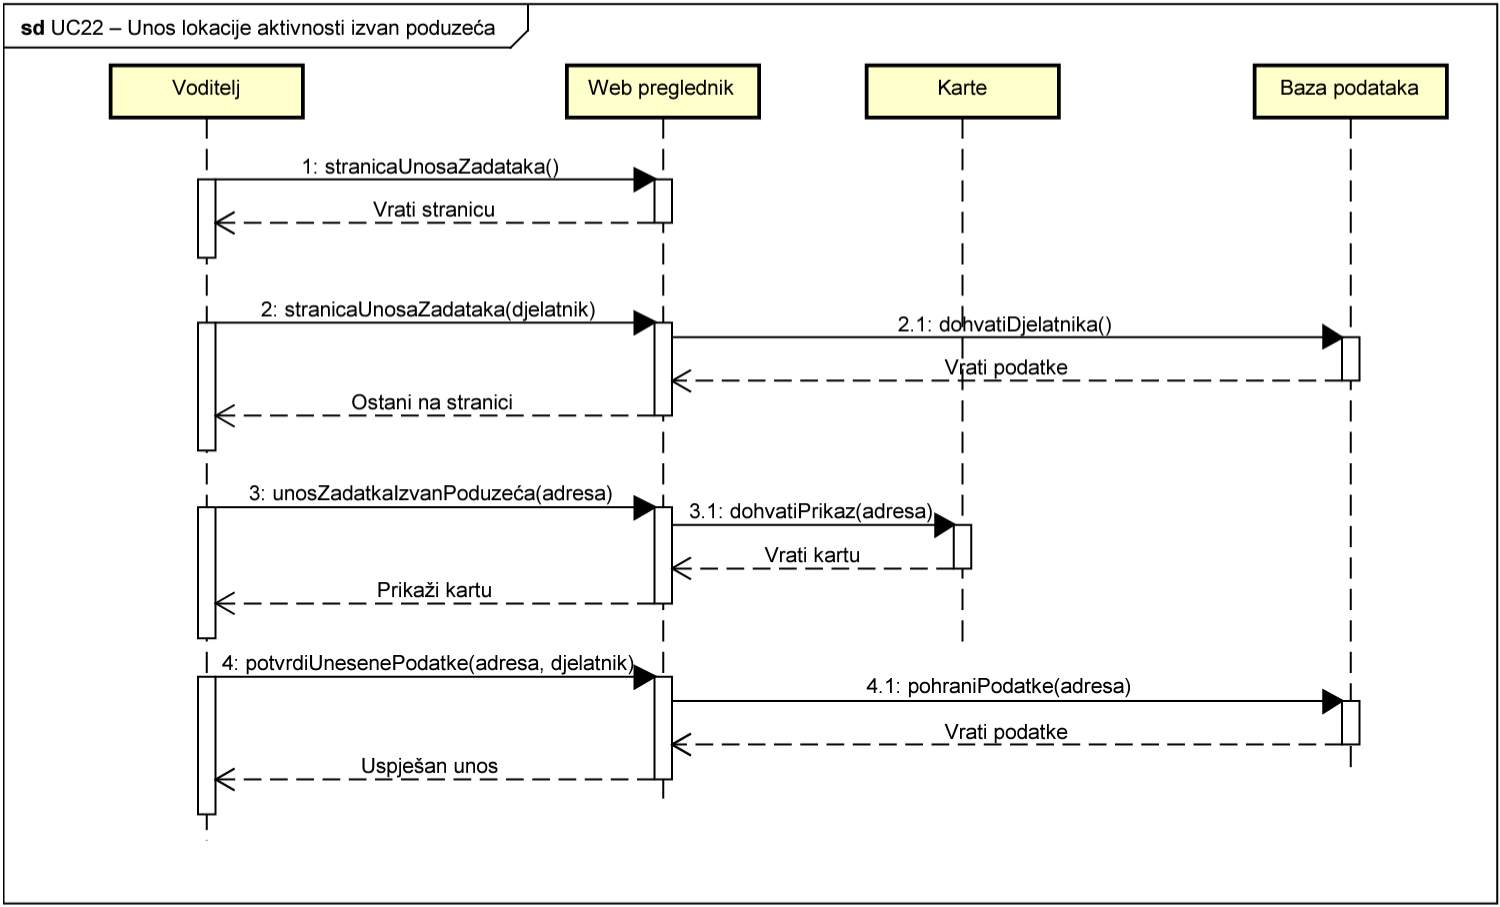
\includegraphics[width=\textwidth]{UC22}
				Slika 3.5 Unos lokacije aktivnosti izvan poduzeća
				\eject
	
		\section{Ostali zahtjevi}
		 	
		 	\noindent Sustav treba:
			 \begin{itemize}
			 	\item omogućiti korištenje hrvatskih dijakritičkih znakova pri unosu i prikazu tekstualnog sadržaja
			 	\item podržati višekorisnički rad u realnom vremenu
			 	\item dati odgovor na traženi upit unutar nekoliko sekundi kada se dohvaćaju podaci iz baze podataka
			 	\item imati intuitivno i jednostavno za korištenje korisničko sučelje
			 	\item biti implementiran kao web aplikacija koristeći objektno-orijentirane jezike
			 	\item neispravno korištenje korisničkog sučelja ne smije narušiti rad sustava
			 	\item osigurati sigurnu, brzu i otpornu na vanjske greške vezu s bazom podataka
			 \end{itemize}
			 
			 
			 
	